\glsresetall{} 
\chapter{Operations Concepts}

\lettrine[lines=2, findent=0pt, nindent=5pt]{B}{} efore discussing the
\gls{pops} it is necessary to go over basic terminology. Without doing so, it
may become very easy for descriptions to become unclear or imprecise. Some of
these terms have been illustrated in Figure \ref{fig:terminology}

\section{General Definitions}

\begin{description} 

    \item[Ephemeris] is a time series of orbital state vectors in a given
	coordinate system. These state vectors have a position component,
	$\sev{r}$, a velocity component, $\sev{v}$, and an epoch for each
	vector, $e$. See section \ref{sgp4_section} for a more detailed
	discussion on ephemerides.

    \item[Area of Interest] An \gls{aoi} is a region on the Earth that is of
	some particular importance to an operator. It is the region in which
	one or more spacecraft should observe through some means. \glspl{aoi}
	can be specified as a point location, an area target, or a latitude
	range. Some examples of \glspl{aoi} are illustrated in \ref{fig:AOIs}.

    \item[Field of View] The \gls{fov} is the extent to which a sensor or
	instrument may observe the outside world at a given time. The size and
	shape of an \gls{fov} varies based on the design of the sensor or
	instrument. \glspl{fov} can theoretically describe any volume of space
	but, for the purposes of this thesis, it may be assumed that they are
	conical. Specifically, the \gls{fov} is defined by a single half-angle,
	$\theta$. Suppose an instrument is pointing along some vector,
	$\sev{u}$. Let us define another vector, $\sev{v}$ such that the angle
	between it and $\sev{u}$ is $\theta$. The \gls{fov} is the volume
	described by rotating $\sev{u}$ around $\sev{v}$.


    \item[Field of Regard] The \gls{for} is similar to the \gls{fov} but
	instead of being the area a sensor can observe in a single time
	instant, the \gls{for} is the volume of space a sensor can possibly
	observe by changing its orientation. Typically, it is constrained by
	some physical or operational constraint. It is not possible to observe
	the entire \gls{for}; Rather, only a subset of the \gls{for} can be
	observed. This subset is the instrument's \gls{fov}.  For example, let
	us consider an optical sensor fixed to a spacecraft orbiting the earth.
	The position of the sensor at particular time instant is given by the
	spacecraft's orbit and cannot be changed unless a propulsive manoeuvre
	is performed.  Of course, the position of sensor can be changed
	slightly by changing the attitude of the spacecraft, since the
	instrument is most likely not located at the spacecraft's centre of
	mass. But, this can be ignored since the distance the instrument can
	translate is negligible compared to its orbit.  Conversely, The
	orientation of the instrument can be changed, and this has a meaningful
	effect on the \gls{for}. If no constraints are put on the attitude of
	the spacecraft, the \gls{for} is everywhere, since the instrument can
	be pointed in any direction. This is not always true though so let us
	say the spacecraft can only point an angle, $\alpha$, off nadir.  The
	\gls{for} would then be the cone described by the half-angle $\alpha +
	\theta$, where $\theta$ is again the half-angle of the conical sensor.
	Figure \ref{fig:fovfor} for an illustration of this example.  The
	larger blue cone is the \gls{for}. The red cone is the sensor's actual
	\gls{fov}. Its boresight is offset from the blue cone's.


\begin{figure} 
    \centering
    \begin{minipage}[c]{0.45\textwidth}
	\centering
	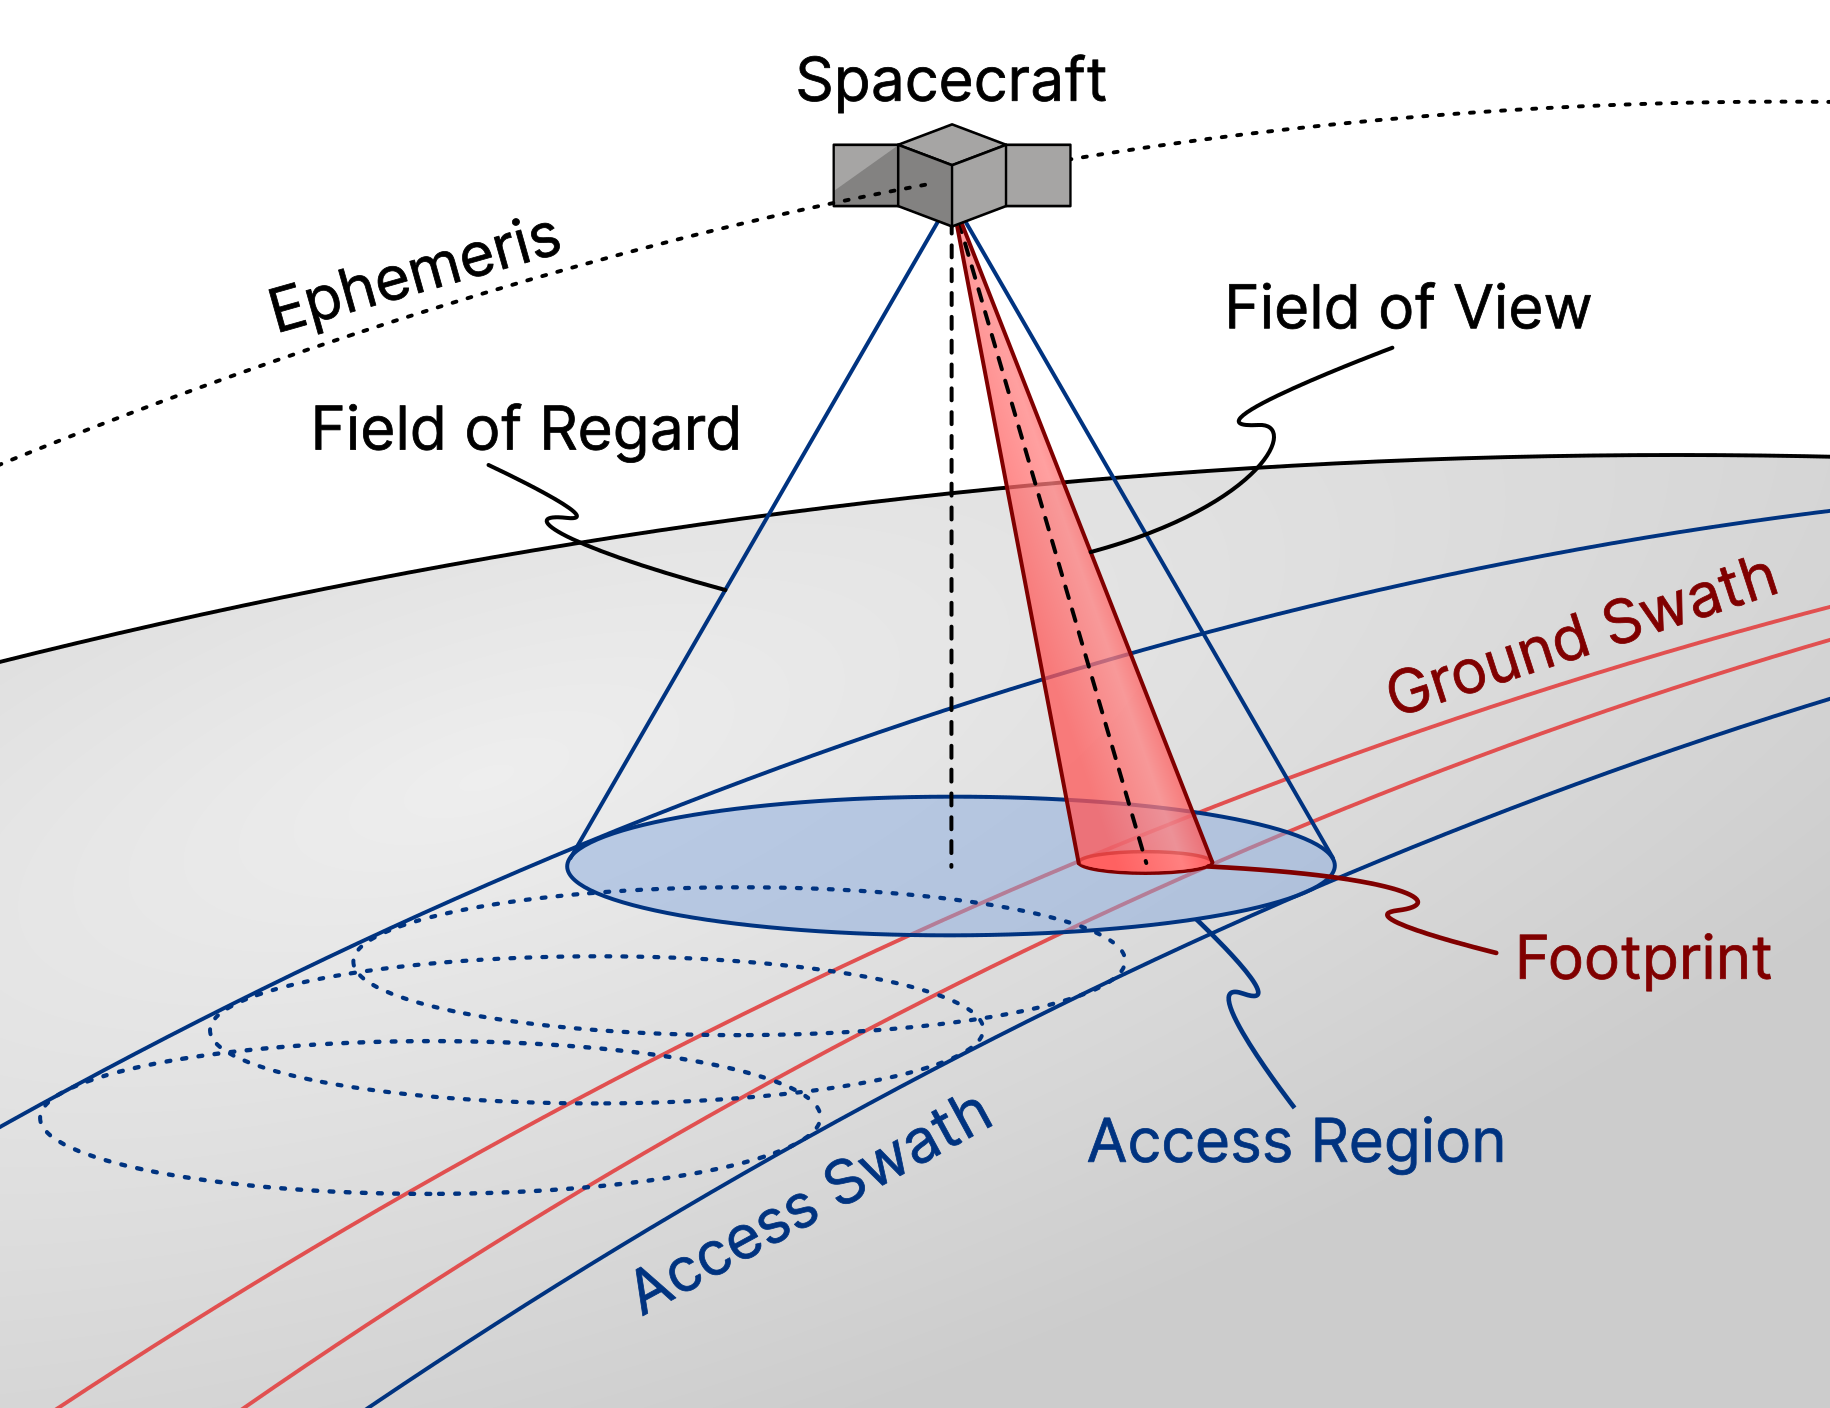
\includegraphics[width=\textwidth]{terminology.png} 
	\caption{General Illustration of Terminology}
	\label{fig:terminology} 
    \end{minipage}
    \hfill
    \begin{minipage}[c]{0.45\textwidth}
	\centering
	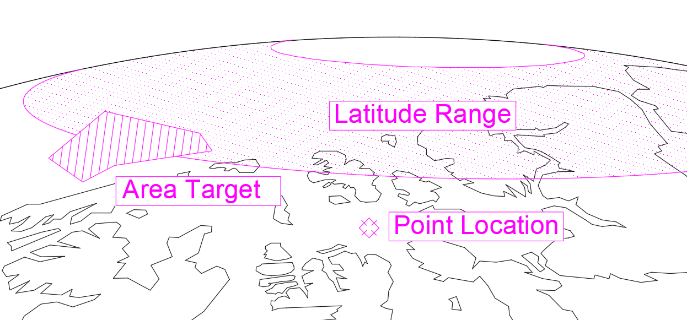
\includegraphics[width=\textwidth]{AOIs.png} 
	\caption{Different Types of Areas of Interest}
	\label{fig:AOIs} 
    \end{minipage} 
\end{figure}

    \item[Footprint] The footprint is the area on Earth that can be observed by
	an instrument's \gls{fov} or \gls{for} at a given time. It can be found
	by intersecting the \gls{fov} or \gls{for} with the surface of the
	Earth.  These intersection points form a boundary and the enclosed area
	within this boundary is the footprint. For clarity, it should be
	assumed that footprint refers to an \gls{for}'s footprint, unless
	otherwise specified.

    \item[Swath] If a sensor is moving over time, its footprint will move with
	it. A swath is the union of all footprints over a time range.  It is
	the region on Earth that can be possibly observed at some point by the
	sensor.

    \item[Horizon Swath] A horizon swath is a special case where the entire
	Earth is within the sensor's \gls{for}. This may be true for certain
	\gls{rf} payloads. In this case, the sensor can only `see' up until the
	horizon. That is, the `horizon' footprint is all of the points on Earth
	whose tangent line intersects with the sensor. Again, as the horizon
	footprint moves, this forms the horizon swath.

\end{description}



\section{Time Tag Commands}

At the Space Flight Laboratory (SFL), satellites are commanded through the use
of the Nanosatellite Protocol (NSP). NSP commands are a custom standard
developed by SFL to facilitate ground and intra-satellite communication. They
are designed to minimize the effects of low-bandwidth radio communication links
that are prone to error. These commands handle all aspects of nominal
operation, from turning individual units on or off, to specifying attitude
modes or initiating data transfers. Once a command is sent, it is executed
immediately upon being received. This raises the concern of how can a
spacecraft be commanded when it does not have a direct communication link with
a ground station. To address this, there exist Time Tag Commands (TTCs). TTCs
are NSP commands that have been prepended with a timestamp and a group ID. When
the spacecraft’s system clock reaches the time specified in the timestamp, that
command is executed. The group ID allows operators to group TTCs such that they
may be considered as a collection rather than as separate commands, allowing
for reference or removal as a single unit. TTCs are prepared in advance by an
operator and uploaded in bulk to the spacecraft. This allows operators to
control the spacecraft when direct communication cannot be established.

At the \gls{sfl}, satellites are commanded through the use of the \gls{nsp}.
\gls{nsp} commands are a custom standard developed by \gls{sfl} to facilitate
ground and intra-satellite communication. They are designed to minimize the
effects of low-bandwidth radio communication links that are prone to error.
These commands handle all aspects of nominal operation, from turning individual
components on or off, to specifying attitude modes or initiating data
transfers. Once a command is sent, it is executed immediately upon being
received. This, of course, poses an obvious problem, how should a spacecraft be
commanded when it does not have a direct communication link with a ground
station. To address this, there exist \glspl{ttc}. These are \gls{nsp} commands
that have been prepended with a timestamp. When the spacecraft's internal clock
reaches the time specified in the timestamp, that command is exectuted. These
\glspl{ttc} are prepared in advance by an operator and uploaded in bulk to the
spacecraft. This allows operators to control the spacecraft when direct
communication cannot be established.



